\documentclass[tikz, border=10pt]{standalone}
% cf http://cloford.com/resources/colours/websafe1.htm
\definecolor{sv-all}{RGB}{255,153,255}
\definecolor{sv-gxe-m2}{RGB}{255,204,255}
\definecolor{sv}{RGB}{255,153,255}
\definecolor{m1}{RGB}{153,153,255}
\definecolor{m2}{RGB}{153,255,153}
\definecolor{ge}{RGB}{255,255,153}
\definecolor{sp}{RGB}{255,153,153}
\definecolor{vi}{RGB}{255,204,153}
\definecolor{ma}{RGB}{204,255,153}
\definecolor{hedo}{RGB}{153,153,255}
\definecolor{nap}{RGB}{153,255,153}

\definecolor{level-1}{RGB}{255,204,255}
\definecolor{level-2}{RGB}{153,153,255}
\definecolor{level-3}{RGB}{153,255,153}
\definecolor{level-4}{RGB}{255,255,153}
\definecolor{level-5}{RGB}{255,153,153}
\definecolor{level-6}{RGB}{255,204,153}
\definecolor{level-7}{RGB}{204,255,153}

\usetikzlibrary{
  mindmap,
  decorations.pathreplacing,    % paths with shoapes of curly braces
  positioning,     % positions like above of node
  fit              % legend bounding box fitting all nodes
}
\tikzset{
  node distance=4ex and 4ex,
  % on grid,  % node distance from the centers
  every node/.style = {
    rectangle,
    minimum width=5em,
    minimum height=3ex,
    text depth=1pt,
    draw,
    outer sep = 2pt,
    inner sep = 3pt
  },
  every edge/.style = {->,draw},
  virtual/.append style = {draw=none, circle, minimum width=1em},
  % virtual/.append style = {draw, color=black!50},   % debugging purposes
  several-all/.append style = {fill = sv-all},
  several-gxe-m2/.append style = {fill = sv-gxe-m2},
  m1/.append style = {fill = m1},
  m2/.append style = {fill = m2},
  gxe/.append style = {fill = ge},
  sp/.append style = {fill = sp},
  vi/.append style = {fill = vi},
  ma/.append style = {fill = ma},
  aux/.append style = {fill = none},
  hedo/.append style = {fill = hedo},
  nap/.append style = {fill = nap},
  legendkey/.append style = {minimum width=3ex},
  legendtext/.append style = {draw=none, fill = black!10},
  ->,        % arrows for all
  >=stealth  % arrow type
}
\pgfdeclarelayer{background}
\pgfsetlayers{background,main}


\begin{document}

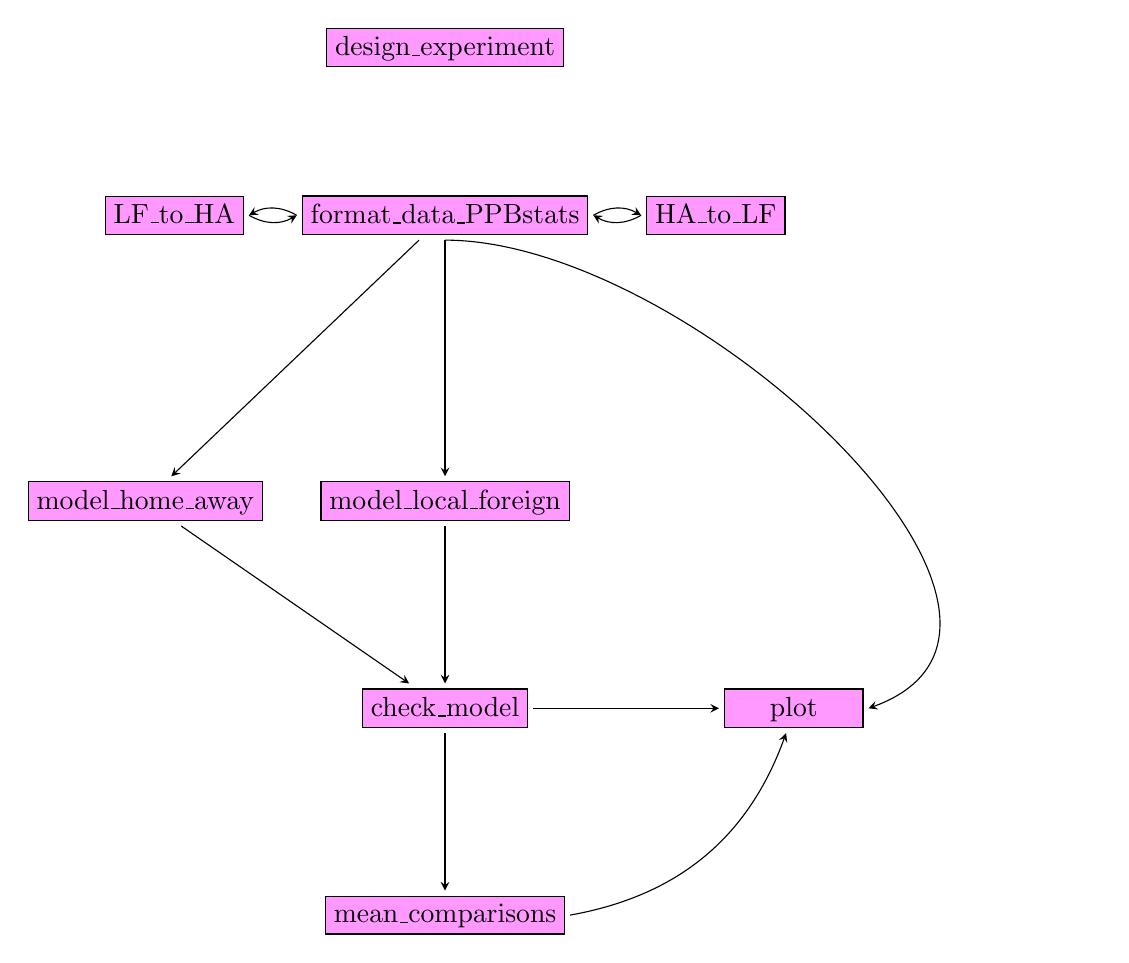
\begin{tikzpicture}

  %% nodes
  \node[several-all] (DE) {design\_experiment};

  \node[several-all] (FD) [below=1.5cm of DE] {format\_data\_PPBstats};
  
  \node[several-all] (HALF) [right=of FD] {HA\_to\_LF};
  \node[several-all] (LFHA) [left=of FD] {LF\_to\_HA};
  
  \node[several-all]  (LF) [below=3cm of FD]  {model\_local\_foreign};
  \node[several-all]   (HA)  [left=of LF] {model\_home\_away};

  \node[several-all] (CM) [below=2cm of LF] {check\_model};

  \node[several-all] (MC) [below=2cm of CM] {mean\_comparisons};

  \node[several-all] (P) [right=of CM, xshift=5em] {plot};


  %% arrows
  \draw (FD.east) to[bend left] (HALF.west);
  \draw (FD.west) to[bend right] (LFHA.east);
  \draw (HALF.west) to[bend left] (FD.east);
  \draw (LFHA.east) to[bend right] (FD.west);
  
  \draw (FD.south) to[out=0,in=20] (P.east);
  \draw (FD) to (HA);
  \draw (FD) to (LF);

  \draw (HA) to (CM);
  \draw (LF) to (CM);

  \draw (CM) to (MC);

  \draw (CM.east) to [left] (P);
  \draw (MC.east) to [bend right] (P);

\end{tikzpicture}

\end{document}
